\begin{exercise}
      {ID-88a4ca5d6db7e361e14af294394530579ad3b560}
      {Fernsehsendung}
  \ifproblem\problem
    Es soll die Beliebtheit einer Fernsehsendung überprüft werden.
    Eine Blitzumfrage lieferte folgendes Ergebnis: \pc{30} der Zuschauer,
    die die Sendung gesehen hatten, waren 25 Jahre und jünger.
    Von diesen hatten \pc{50} und von den übrigen Zuschauern (über 25
    Jahre) hatten \pc{80} eine positive Meinung.
    \begin{enumerate}[a)]
      \item Stelle den Sachzusammenhang in einer Vierfeldertafel dar.
      \item Stelle den Sachzusammenhang in einem Baumdiagramm dar und
            zeichne auch den inversen Baum. Bestimme alle Pfadwahrscheinlichkeiten.
      \item Wie viel Prozent der Zuschauer, von denen man weiß, dass sie
            eine positive Meinung über die Sendung hatten, waren älter
            als 25 Jahre?
      \item Wie viel Prozent der Zuschauer, von denen man weiß, dass sie
            älter als 25 Jahre sind, hatten keine positive Meinung über
            die Sendung?
      \item Überprüfe durch eine Rechnung, ob in diesem Fall \textit{Alter} und
            \textit{Meinung} stochastisch unabhängig sind.
    \end{enumerate}
  \fi
  %\ifoutline\outline
  %\fi
  \ifoutcome\outcome
    \begin{enumerate}[a)]
      \item Der Sachzusammenhang lässt sich z.\,B. auf folgende Weise in
            einer Vierfeldertafel darstellen:
            \begin{center}
              \begin{tabular}{|c||c|c||c|}
                \hline
                         & pos        & neg        & Summe     \\
                \hline
                \hline
                $\leq25$ & \num{0.15} & \num{0.15} & \num{0.3} \\
                \hline
                $>25$    & \num{0.56} & \num{0.14} & \num{0.7} \\
                \hline
                \hline
                Summe    & \num{0.71} & \num{0.29} & \num{1}   \\
                \hline
              \end{tabular}
            \end{center}
      \item Unterscheidet man auf der ertsen Stufe das \emph{Alter} der
            Zuschauer, dann könnte der Baum folgenden Aufbau besitzen:
            \begin{center}
              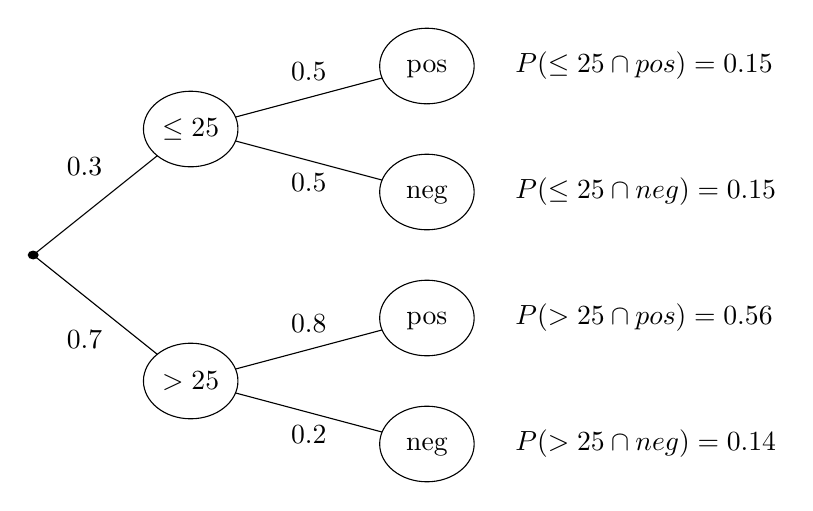
\begin{tikzpicture}[yscale=0.8]
                \coordinate (A) at (0,  0);
                \coordinate (B) at (2,  2);
                \coordinate (C) at (2, -2);
                \coordinate (D) at (5,  3);
                \coordinate (E) at (5,  1);
                \coordinate (F) at (5, -1);
                \coordinate (G) at (5, -3);
                \draw (A) -- node[above left]{\vphantom{$($}\num{0.3}} (B);
                \draw (B) -- node[above]     {\vphantom{$($}\num{0.5}} (D);
                \draw (B) -- node[below]     {\vphantom{$($}\num{0.5}} (E);
                \draw (A) -- node[below left]{\vphantom{$($}\num{0.7}} (C);
                \draw (C) -- node[above]     {\vphantom{$($}\num{0.8}} (F);
                \draw (C) -- node[below]     {\vphantom{$($}\num{0.2}} (G);
                \fill[fill=black] (A) circle[radius=2pt];
                \filldraw[fill=white, draw=black] (B) circle[radius=6mm];
                \filldraw[fill=white, draw=black] (D) circle[radius=6mm];
                \filldraw[fill=white, draw=black] (E) circle[radius=6mm];
                \filldraw[fill=white, draw=black] (C) circle[radius=6mm];
                \filldraw[fill=white, draw=black] (F) circle[radius=6mm];
                \filldraw[fill=white, draw=black] (G) circle[radius=6mm];
                \node at (B) {$\leq25$};
                \node at (D) {\vphantom{$($}pos};
                \node at (E) {\vphantom{$($}neg};
                \node at (C) {$>25$};
                \node at (F) {\vphantom{$($}pos};
                \node at (G) {\vphantom{$($}neg};
                \node[right=1cm] at (D) {$P(\leq25\cap\text{pos})=\num{0.15}$};
                \node[right=1cm] at (E) {$P(\leq25\cap\text{neg})=\num{0.15}$};
                \node[right=1cm] at (F) {$P(>25\cap\text{pos})=\num{0.56}$};
                \node[right=1cm] at (G) {$P(>25\cap\text{neg})=\num{0.14}$};
              \end{tikzpicture}
            \end{center}
            Der inverse Baum dazu hat folgende Gestalt:
            \begin{center}
              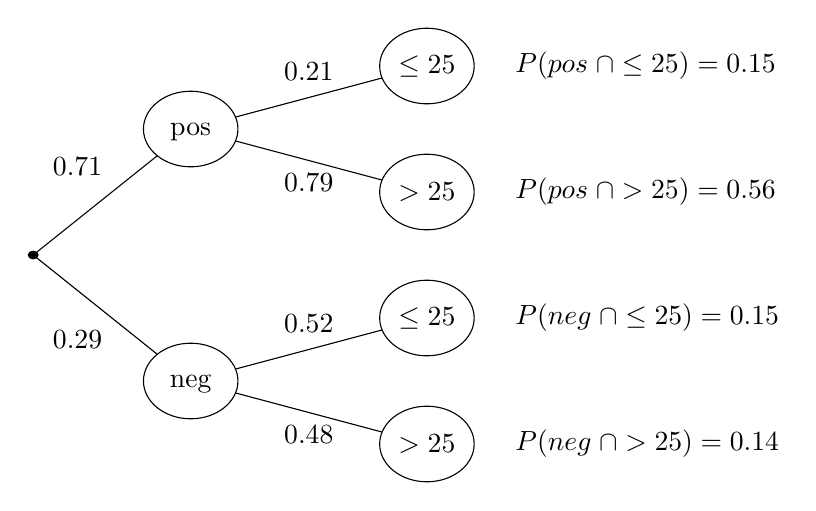
\begin{tikzpicture}[yscale=0.8]
                \coordinate (A) at (0,  0);
                \coordinate (B) at (2,  2);
                \coordinate (C) at (2, -2);
                \coordinate (D) at (5,  3);
                \coordinate (E) at (5,  1);
                \coordinate (F) at (5, -1);
                \coordinate (G) at (5, -3);
                \draw (A) -- node[above left] {\vphantom{$($}\num{0.71}} (B);
                \draw (B) -- node[above]      {\vphantom{$($}\num{0.21}} (D);
                \draw (B) -- node[below]      {\vphantom{$($}\num{0.79}} (E);
                \draw (A) -- node[below left] {\vphantom{$($}\num{0.29}} (C);
                \draw (C) -- node[above]      {\vphantom{$($}\num{0.52}} (F);
                \draw (C) -- node[below]      {\vphantom{$($}\num{0.48}} (G);
                \fill[fill=black] (A) circle[radius=2pt];
                \filldraw[fill=white, draw=black] (B) circle[radius=6mm];
                \filldraw[fill=white, draw=black] (D) circle[radius=6mm];
                \filldraw[fill=white, draw=black] (E) circle[radius=6mm];
                \filldraw[fill=white, draw=black] (C) circle[radius=6mm];
                \filldraw[fill=white, draw=black] (F) circle[radius=6mm];
                \filldraw[fill=white, draw=black] (G) circle[radius=6mm];
                \node at (B) {\vphantom{$($}pos};
                \node at (D) {$\leq25$};
                \node at (E) {$>25$};
                \node at (C) {\vphantom{$($}neg};
                \node at (F) {$\leq25$};
                \node at (G) {$>25$};
                \node[right=1cm] at (D) {$P(\text{pos\;}\cap\leq25)=\num{0.15}$};
                \node[right=1cm] at (E) {$P(\text{pos\;}\cap>25)=\num{0.56}$};
                \node[right=1cm] at (F) {$P(\text{neg\;}\cap\leq25)=\num{0.15}$};
                \node[right=1cm] at (G) {$P(\text{neg\;}\cap>25)=\num{0.14}$};
              \end{tikzpicture}
            \end{center}
      \item Etwa \pc{79} der Zuschauer, von denen man weiß, dass sie eine
            positive Meinung über die Sendung hatten, waren älter als
            25 Jahre.
      \item Etwa \pc{20} der Zuschauer, von denen man weiß, dass sie
            älter als 25 Jahre sind, hatten keine positive Meinung über
            die Sendung.
      \item Die beiden Merkmale \emph{Alter} und \emph{Meinung} sind
            stochastisch abhängig, denn es gilt:
            \begin{equation*}
              P(\leq25\cap\text{pos})
              =\num{0.15}
              \neq\num{0.213}
              =\num{0.3}\cdot\num{0.71}
              =P(\leq25)\cdot P(\text{pos})
            \end{equation*}
    \end{enumerate}
  \fi
\end{exercise}
